\documentclass[9pt,conference,a4paper]{IEEEtran}
\IEEEoverridecommandlockouts

\usepackage{graphicx}


\title{Particle Swarm Optimization in Multi-Tensor Imaging.}
\author{
	\IEEEauthorblockN{
		Michael Paquette\IEEEauthorrefmark{1},
		Eleftherios Garyfallidis\IEEEauthorrefmark{1},
		Samuel St-Jean\IEEEauthorrefmark{1},
		Pierrick Coup\'e\IEEEauthorrefmark{2},
		Maxime Descoteaux\IEEEauthorrefmark{1}
	}

	\IEEEauthorblockA{\IEEEauthorrefmark{1} Sherbrooke Connectivity Imaging Lab (SCIL), Computer Science Department, Universit\'e de Sherbrooke, Sherbrooke, Canada}
	\IEEEauthorblockA{\IEEEauthorrefmark{2} CNRS Laboratoire Bordelais de Recherche en Informatique (LaBRI), Bordeaux, France}

%	\thanks{This work is supported by your Mom}
}




\begin{document}
\maketitle

For the ISBI HARDI reconstruction challenge 2013 we developed a local estimation method based Multi-Tensor (MT) fitting with the Particle Swarm Optimization technique (PSO) \cite{kennedy-russell:95}. 
We apply this reconstruction to the DTI and HARDI data categories. 

\bigskip

To fit a MT to the diffusion signal $S = \{S_k\}_{k=0}^M$ with gradient scheme $ \{b_k, g_k\}_{k=0}^M$ is to find some parameters so that $y = \{y_k\}_{k=0}^M$, $y_k = \sum_{i=0}^N f_i e^{-b_k g_k^t D_i g_k}$ resemble the measured signal $S$, where $g_k$ is the k$^{th}$ normalized gradient wavevector and $b_k$ the corresponding b-value, $D_i$ is a rank 2 symmetric tensor with volume fraction $f_i$ and $N$ is the number of compartment in the fit.

\bigskip

To perform the MT fitting, we minimize the fitting error for some cost function, here the squared error between the measured signal and the MT approximation, $ \| S-y \|_2 $. 
This minimization is carried on by the particle swarm optimization. The PSO is a stochastic optimization algorithm using population interaction to find the minimum of a function $ f: \mathbf{R}^n \rightarrow \mathbf{R} $. 
It starts by randomly initiating $Np$ particles and $Np$ velocities: points $\Omega^0_j \in \mathbf{R}^n$ and $v^1_j \in \mathbf{R}^n$. 
These points then evolve into the search space according to $\Omega^{t+1}_j = \Omega^t_j + v^{t+1}_j$ and $ v^{t+1}_j = w v^t_j + \phi_p r_p (p^{t}_j - \Omega^t_j) + \phi_g r_g (g^t - \Omega^t_j)$ where $w$, $\phi_p$ and $\phi_g$ are user tuned parameters, $p^t_j$ is the $j^{th}$ particle's best known position at iteration $t$, $g^t$ is the swarm's best known position at iteration $t$ and $r_p,r_g \sim \mathcal{U}[0,1]$. 
The process is repeated for $Ni$ iteration or until some convergence criterion is met. 
The velocity update formula means that the particles are drawn to swarm's best known position while been deflected by their own best location and conserving some of their past momentum. 
Particles near $g$ will fully explore that area of the space and find the true local minimum while others will converge there from all over the space, allowing to potentially find new attractor points or finding a better values near their own best known location. 
Finally, the conservation of their previous velocity and it's random weighting with $p$ and $g$ allows for the particles to escape non-optimal local minimum, potentially attracting to them other particles that are stuck.

\bigskip

For the contest, we compared using the raw DW, the DW denoised with nonlocal means a rician noise model and denoised with adaptive nonlocal means \cite{manjon-coupe:10} using a rician noise model. 
As proposed in \cite{descoteaux-wiest-daessle-etal:08}, each DW images were processed independently. 

We constrained the MT model to use only prolate tensors and also tested adding an isotropic compartment and fixing the volume fraction to be equal between the non-isotropic compartment.

Since the number of compartment is a meta parameter, we chose as a strategy to overfit at every voxel by always estimating three fiber compartment and to re-estimate with less compartment certain voxels based on two criterion.
We first enforce that no voxel has peaks closer to each other than $\theta^\circ$.
This angular based pruning provide a good cleaning because the peaks tends to converge together when the voxel is been overmodeled.
The only drawback is that we put a hard lower bound on the methods angular resolution.
Secondly, we look at the model complexity of neighboring voxel after the angular pruning to detect outlier. 
A voxel that has more compartment than $\Psi$\% of it's neighborhood is re-estimated with less compartment.

In order to validate which denoising and MT constraints were optimal on the training data, we computed tractography for all the different combination.
Considering that the given ground truth was a binary connectivity matrix with given ROI, we generated connectivity matrix from track count and used them to qualitatively evaluate each method.
For a specific threshold, we can binarize our matrix and obtain a connectivity error, $\#$ false connections + $\#$ missing connections, where a false connection is two regions considered connected for that threshold that are not in the ground truth and a missing connection is two regions not considered connected for that threshold that are in the ground truth.
Looking at that error for different threshold gives an overview of the validity of the tractogram produced from that method.
Indeed, a good tractogram should allow for a large range of threshold value that gives low connectivity matrix error.

\bigskip

For the final result, for both the DTI dataset (32 directions at b = 1200 s/mm$^2$) and the HARDI dataset (64 directions at b = 3000 s/mm$^2$), we used the denoising from \cite{manjon-coupe:10} for snr 10 and 20 and no denoising for snr 30. The MT model fitted had three prolate tensors and one isotropic tensor with fixed equal volume fractions. 
The pruning parameters were $\theta = 30^\circ$, $\Psi = 50$\% for DTI and $\theta = 20^\circ$, $\Psi = 50$\% for HARDI.




\begin{figure}
\centering
\begin{tabular}{c  c}
	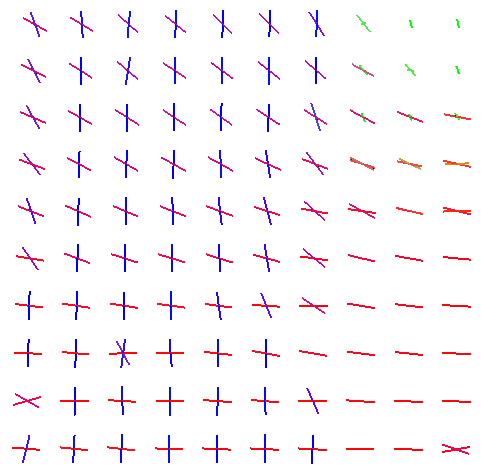
\includegraphics[width=40mm,height=40mm]{dti_slice=22_sel=33_NC=3_iso=1_fr=0_snr=10_type=6_white.png} & 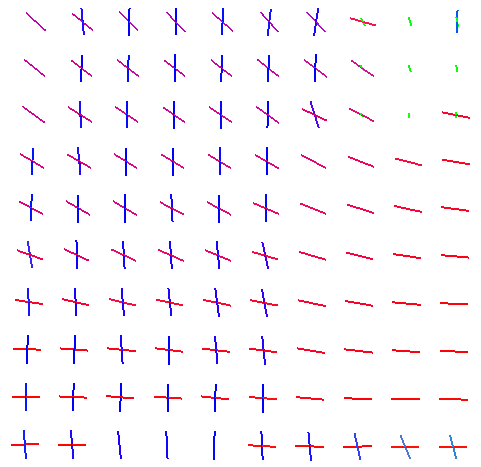
\includegraphics[width=40mm,height=40mm]{hardi_slice=22_sel=33_NC=3_iso=1_fr=0_snr=10_type=6_white.png}\\
\end{tabular}
\caption{Peaks in the testing dataset (ROI = [14:23, 22, 34:43]). Left is DTI, right is HARDI, both result on snr = 10 with denoising from \cite{manjon-coupe:10}}
\end{figure}

%meaning that, as the threshold grow, false bundle disappear faster than true bundle and as the threshold goes down, missing bundle appear faster than new false bundle.



%
%We then launch PSO with with N = 4, with one of those compartment been isotropic. We also fit tensor with $\lambda_2 = \lambda_3$ and $\lambda_1 > \lambda_2$, giving us two eigenvalues and two rotation angles per fiber compartment, one eigenvalue for the isotropic compartment and a volume fraction between the isotropic part and the reste, 14 parameters. We assume that all non-isotropic compartment have equal volume fractions.
%
%From that fit, we extract three peaks. If any voxel has peaks closer to each other than $\theta^\circ$ (e.g. 30$^\circ$), that voxel is re-estimated with one less fiber compartment. This "pruning" provide a good cleaning of the huge overfitting caused because, the peaks tends to converge together when the voxel is been overmodeled, thanks to the isotropic compartment. The only drawback is that we put a hard lower bound on the methods angular resolution ($\theta^\circ$).

%After the angular based model reduction, we further fix the overfitting problem (caused by fitting a fixed number of compartment) by looking at the model complexity of neighbooring voxel to prune outlier based on a simple threshold (we re-fit with one less fiber compartment if a voxel is more complex than H\% of it's one-voxel neighboorhood)


%Hello \cite{manjon-coupe:10}, \cite{descoteaux-deriche-etal:09}, \cite{Descoteaux2008}, \cite{tournier-calamante-etal:07}.


\bibliographystyle{ieeetr}
\bibliography{/media/Data/work/scil-bibtex/scilBibTex.bib}

\
\end{document}


